\section{The PID Python Libraries}

Most of PID python libraries had been developed base on the Arduino PID and series blog by Beauregard \cite{Arduino_PID}  \cite{Improving_PID}. The Arduino version has been updated by 
Gelraen \cite{Arduino_PID_V2} on January 2021.

\subsection{Python packages.}
% \textbf{}
This subsection will give a quick overview on the most use python packages.

\textbf{Simple PID} \cite{Simple_Pid} follow the guideline implementation by Brett Beauregard  \cite{Improving_PID}. The package has included the windup protection, the derivative kick avoidance, online parameters tuning, smooth controller transition from Auto (PID on) to manual. The last update was on 17 November 2020

\textbf{ivPID} \cite{ivPID} PID controller implementation base on equation [\ref{eqn:4}] with windup protection. This package does not has derivative kick avoidance or smooth controller switching.

\textbf{DvG${\_}$PID${\_}$Controller} \cite{DvG_PID_Controller}: another Arduino library \cite{Arduino_PID} ported to Python by Dennis van Gils (a senior research of Twente University) in july 2020. This package has include all functionality from Arduino library ( windup protection, derivative kick, controller switch, bumpless transfer).

\subsection{PID design example with Jupiter notebook}

There are many other PID controller example had been written in python. A few more example are mentioned below:

An explanation on PID controller and python implementation can be found in \href{https://apmonitor.com/pdc/index.php/Main/ProportionalIntegralDerivative}{apmonitor dynamic and control website}.

\begin{figure}[H]
	\centering
	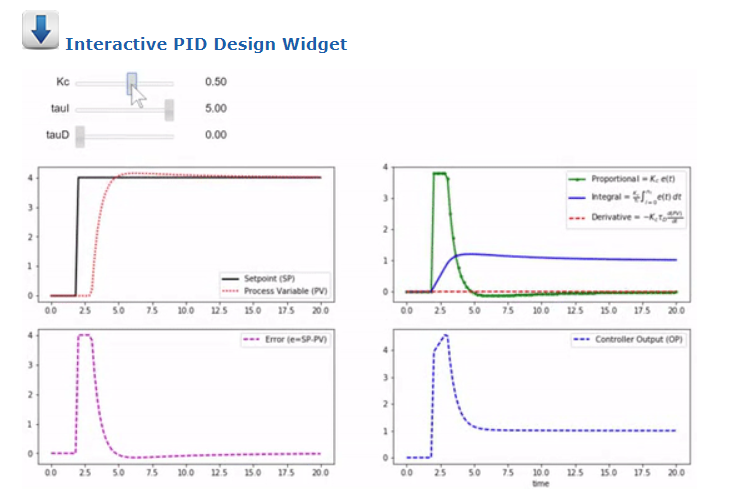
\includegraphics[width=0.8\columnwidth]{Pictures/PID_interactive.png}
	\caption[Short title]{Pid interactive notebook on apmonitor}
	\label{figure:interactive notebook}
\end{figure}

\newpage

A Jupyter/Python notebooks series on PID controller on (chapter 4) chemical process course of Notre Dame University\cite{CBE}.

\begin{figure}[H]
	\centering
	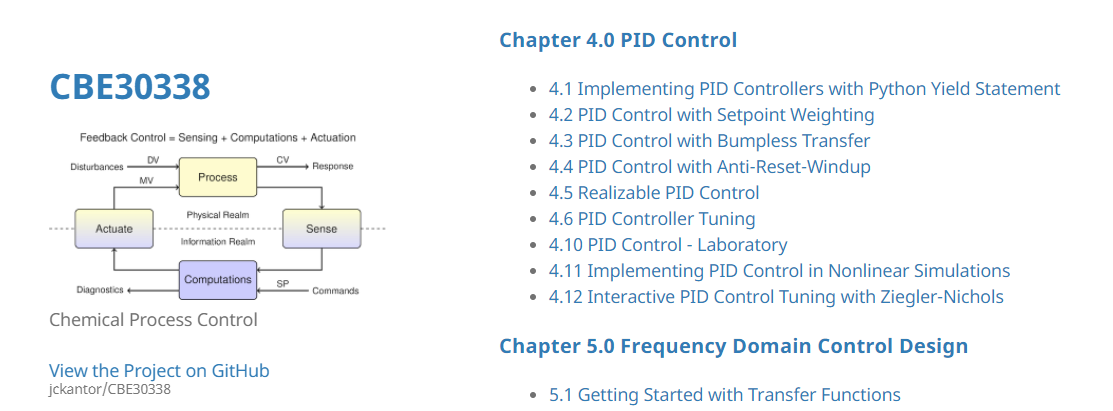
\includegraphics[width=0.8\columnwidth]{Pictures/PID_NotreDame.png}
	\caption[Short title]{Pid controller notebook series of Notre Dame University chemical process course.}
	\label{figure:NotreDame notebook}
\end{figure}

\newpage